\documentclass{beamer}

\usepackage{amsmath}
\usepackage{xspace}


% \newcommand\doubleplus{+\kern-1.3ex+\kern0.8ex}
\newcommand\doubleplus{\ensuremath{\mathbin{+\mkern-10mu+}}}


%% oracles
\newcommand{\ora}[1]{\ensuremath{\mathcal{O}\mathsf{#1}}\xspace}
\newcommand{\oramsg}[1]{\ensuremath{\mathsf{#1}}\xspace}
%% algorithm
\newcommand{\algo}[1]{{\textsc{#1}}}
%%primitive algo
\newcommand{\primalgo}[1]{{\ensuremath{\mathsf{#1}}}\xspace}
%%primitive
\newcommand{\prim}[1]{{\ensuremath{\mathsf{#1}}}\xspace}
%%set
\newcommand{\setsym}[1]{{\ensuremath{\mathcal{#1}}}}
%%array
\newcommand{\arraysym}[1]{{\ensuremath{\mathsf{#1}}}}

\newcommand\N{\mathbb{N}}
\newcommand\F{\mathbb{F}}
% \newcommand\Gr{\mathbb{G}}


\def\mathperiod{.}
\def\mathcomma{,}



\newcommand*\set[1]{\{ #1 \}} % in text, we don't want {} to grow
\newcommand*\Set[1]{\left\{ #1 \right\}}
\newcommand*\setst[2]{\{ #1 | #2 \}}
\newcommand*\Setst[2]%
        {\left\{\,#1\vphantom{#2} \;\right|\left. #2 \vphantom{#1}\,\right\}}
% ``set such that''; puts in a vertical bar of the right height


\providecommand{\bin}{\ensuremath{\{0,1\}}\xspace}


% https://tex.stackexchange.com/questions/471713/is-mathrel-always-needed
% https://tex.stackexchange.com/questions/418740/how-to-write-left-arrow-with-a-dollar-sign/626086#626086
\makeatletter
\providecommand\leftsample{\leftarrow\mathrel{\mkern-2.0mu}\pc@smalldollar}
\providecommand\rightsample{\pc@smalldollar\mathrel{\mkern-2.0mu}\rightarrow}
%
\newcommand{\pc@smalldollar}{\mathrel{\mathpalette\pc@small@dollar\relax}}
\newcommand{\pc@small@dollar}[2]{%
  \vcenter{\hbox{%
    $#1\textnormal{\fontsize{0.7\dimexpr\f@size pt}{0}\selectfont\$\hskip-0.05em
 plus 0.5em}$%
  }}%
}
\makeatother


\newcommand{\KeyGen}{\primalgo{KeyGen}}

% Why was this \prim before?
\newcommand{\VRF}{\primalgo{VRF}} 
\newcommand{\rVRF}{\primalgo{rVRF}} 

\newcommand{\Sign}{\primalgo{Sign}}
\newcommand{\Verify}{\primalgo{Verify}}
\newcommand{\Eval}{\primalgo{Eval}}
\newcommand{\Prove}{\primalgo{Prove}}
\newcommand{\Simulate}{\primalgo{Simulate}}
\newcommand{\Extract}{\primalgo{Extract}}


\newcommand{\In}{\primalgo{In}} 
\newcommand{\Out}{\primalgo{Out}} 
\newcommand{\PreOut}{\ensuremath{\primalgo{Out}_0}\xspace} 

\newcommand{\vk}{\ensuremath{\mathsf{vk}}\xspace}
\newcommand{\sk}{\ensuremath{\mathsf{sk}}\xspace}
\newcommand{\pk}{\ensuremath{\mathsf{pk}}\xspace}
\newcommand{\apk}{\ensuremath{\mathsf{apk}}\xspace}
\newcommand{\pkring}{\ensuremath{\setsym{PK}}}
\newcommand{\msg}{\ensuremath{\mathsf{msg}}\xspace}
\newcommand{\aux}{\ensuremath{\mathsf{aux}}\xspace}
\newcommand{\ctx}{\ensuremath{\mathsf{ctx}}\xspace}
\newcommand{\ringset}{\ensuremath{\mathsf{ring}}\xspace}



\newcommand\SNARK{\primalgo{SNARK}}
\newcommand\NIZK{\primalgo{NIZK}}


\newcommand{\adv}{\ensuremath{\mathcal{A}}\xspace}

\endinput

\newcommand{\evalprove}{\primalgo{EvalProve}}
\newcommand{\link}{{\primalgo{Link}}}
\newcommand{\update}{{\primalgo{Update}}}
\newcommand{\hashG}{\primalgo{H}_{\GG}}
\newcommand{\secreteval}{\primalgo{Secret}\eval}
\newcommand{\secretprove}{\primalgo{Secret}\prove}
\newcommand{\secretverify}{\primalgo{Secret}\verify}

\newcommand{\randsel}[0]{\ensuremath{\xleftarrow{\text{\$}}}}
\newcommand{\rel}{\ensuremath{\mathcal{R}}}


\endinput




\newcommand{\skvrf}{\ensuremath{\sk^{\mathsf{vrf}}}}
\newcommand{\pkvrf}{\ensuremath{\pk^{\mathsf{vrf}}}}
\newcommand{\skrvrf}{\ensuremath{\sk^{\mathsf{rvrf}}}}
\newcommand{\pkrvrf}{\ensuremath{\pk^{\mathsf{rvrf}}}}
\newcommand{\sksign}{\ensuremath{\sk^{\mathsf{sign}}}}
\newcommand{\pksign}{\ensuremath{\pk^{\mathsf{sign}}}}
\newcommand{\skksign}{\ensuremath{\sk^{\mathsf{kesign}}}}
\newcommand{\pkksign}{\ensuremath{\pk^{\mathsf{kesign}}}}
\newcommand{\pkssale}{\ensuremath{\pk^{\mathsf{ssale}}}}
\newcommand{\D}{\ensuremath{\Delta}}
\newcommand{\skzkvrf}{\ensuremath{\sk^{\mathsf{zkvrf}}}}
\newcommand{\pkzkvrf}{\ensuremath{\pk^{\mathsf{zkvrf}}}}


\def\comring{\ensuremath{\mathsf{comring}}\xspace}
\def\compk{\ensuremath{\mathsf{compk}}\xspace}


\title{ZK proofs in the polkadot ecosystem} % directions for

\author{Jeffrey Burdges} % \and Alistair Stewart}
\date{26 June 2023}


\begin{document}


\maketitle


\begin{frame}

Polkadot is largely a story of high level optimizations, \\

\hspace{5pt} requiring some understanding of the larger design space. \\ \bigskip

% Examples:
% Grandpa
% Politeness
% NPoS & slashing
% Babe & Sassafras
% 1d Reed-Solomn
%   AFFT + formal derivatives

Also an ambitious but grounded approach to formal security.

% Examples:
% Gav's polakdot paper was an optimistic roll up
% Approvals
%   Assignments by VRF
%   Two phase inclusion

\end{frame}


\begin{frame}{Coming soon}

Hostcalls for some elliptic curves: \\ \smallskip

\hspace{5pt} Bandersnatch, et al. --- single \& multi-scalar multiplication \\

\hspace{5pt} BLS12-381, BLS12-377, BW6-761, BW6-767, BN254 --- \\
\hspace{10pt}  Same, plus multi-miller loop \& final exponentiation \\ 

\bigskip % \bigskip

Afaik any crate for said curve could be adapted becuase \\
we balanced WASM and native elliptic curve arithemtic concerns

\bigskip\bigskip
% \end{frame}
% \begin{frame}

EIP-2537 (BLS12-381) adds 9 calls:  \\ \smallskip

\hspace{5pt} Additions \& hash-to-curves appear unecessary. \\

\hspace{5pt} Groth16 needs 4 pairings \\

\end{frame}


\begin{frame}

What are the high level optimizations in zero knowledge?

\bigskip\bigskip

\hspace{20pt} Just choose the problem you wish to solve!

% Example: Jubjub

\end{frame}


\begin{frame}{web3sum bridges}

Alistair \& Sergey's web3sum BLS protocol sums elliptic curve points,
% \\ \hspace{5pt}
given by a polynomial commitment and optional bitfield. \\

% \bigskip\bigskip

% It maybe faster to add the points yourself if you know the validators

\end{frame}


\begin{frame}{Ring VRFs}

Ring signatures prove the actual signer exists in \\
\hspace{5pt} some publicly specified list, known as the ring.

\bigskip\bigskip

Examples: \\
\hspace{5pt}  Some deniable key exchanges. \\
\hspace{5pt}  Monero, ZCash, etc. are linkable. 

\medskip

Non-examples:  Anonymized certificates, ala COVID.

\bigskip\bigskip

Ring can be a fancy set commitment like ZCash, \\
\hspace{5pt} but membership proofs are always very expensive.
	
\end{frame}



\begin{frame}{ring VRFs}

A verifiable random function (VRF) proves evaluation of a pseudo-random function (PRF) determined by a signing key.

\bigskip\bigskip

Ring VRF is a ring signature that's also a VRF.

\bigskip

A ring verifiable random function (ring VRF) is a ring signature that proves evaluation of a pseudo-random function (PRF) determined by the actual key pair.

\end{frame}


\begin{frame}{Ring VRFs: Sassafras}

Sassafras:  Aura but schedule slots anonymously. \\ \medskip

Anonymity provided by web3sum ring VRF \\
\hspace{5pt}  (or Jet KZK ring VRF or IPP ring VRF or schuffle) \\ \medskip

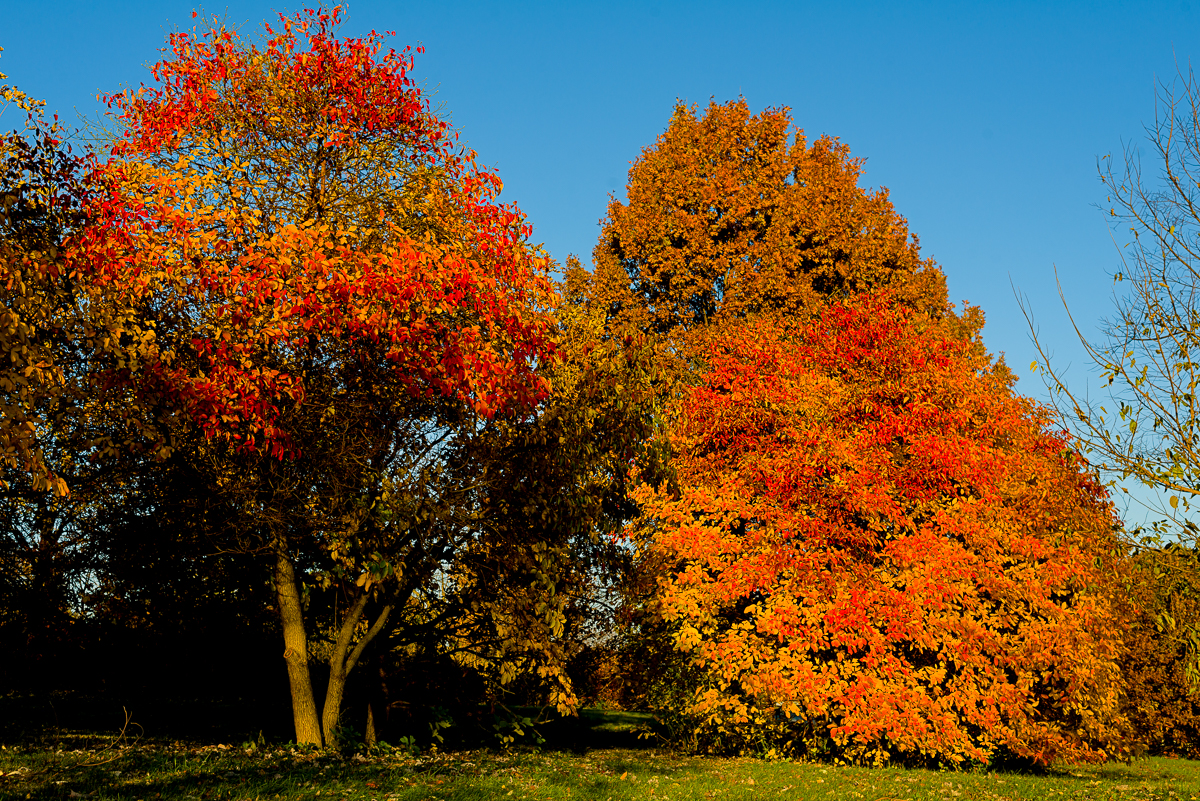
\includegraphics[width=0.8 \textwidth]{../zksummit/Sassafras-albidum.jpg}

Imagine each upcoming slot has a Tor {\tt .onion} URL!

\end{frame}


\begin{frame}{ring VRFs: Special G, Jet KZG, etc}

Zero-knowledge continuations..

\bigskip
	
Q: What are the fastest/cheapest SNARK proofs?
	
\bigskip
	
A: Ones we reuse without reproving.
	
\end{frame}


\begin{frame}{Ring VRFs: Identity}

Anonymity provided by Jet KZK ring VRF \\
\hspace{5pt}  (or maybe Special G ring VRF) \\ \bigskip\bigskip

Imagine this workflow: \\ \medskip
\hspace{5pt} Users scan their epassport on Android Polkadot Vault \\
\hspace{10pt} which registers you a fresh public key on a parachain. \\ \medskip
\hspace{5pt} User anonymously proves their uniqueness to any other parachain \\
\hspace{10pt} Very fast.  Very cheap aka no messages.  \\

\end{frame}


\begin{frame}

% black_FRONT050.png

\begin{columns}
	\begin{column}[t]{0.1\textwidth}
	\end{column}
	\begin{column}[t]{0.3\textwidth}
		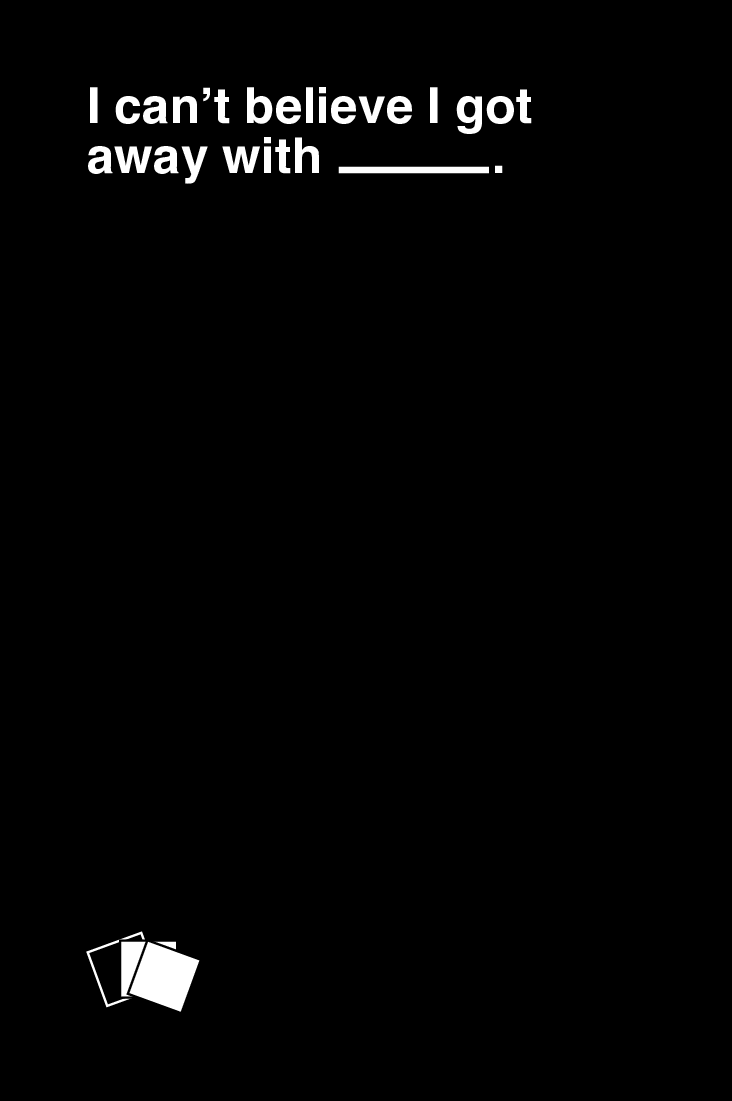
\includegraphics[width=.9\textwidth]{../zksummit/black_FRONT012.png} % {CAC/PNGs-to-print/individual-cards/black_FRONT012.png}
	\end{column}
	\begin{column}[t]{0.3\textwidth}
		\frame{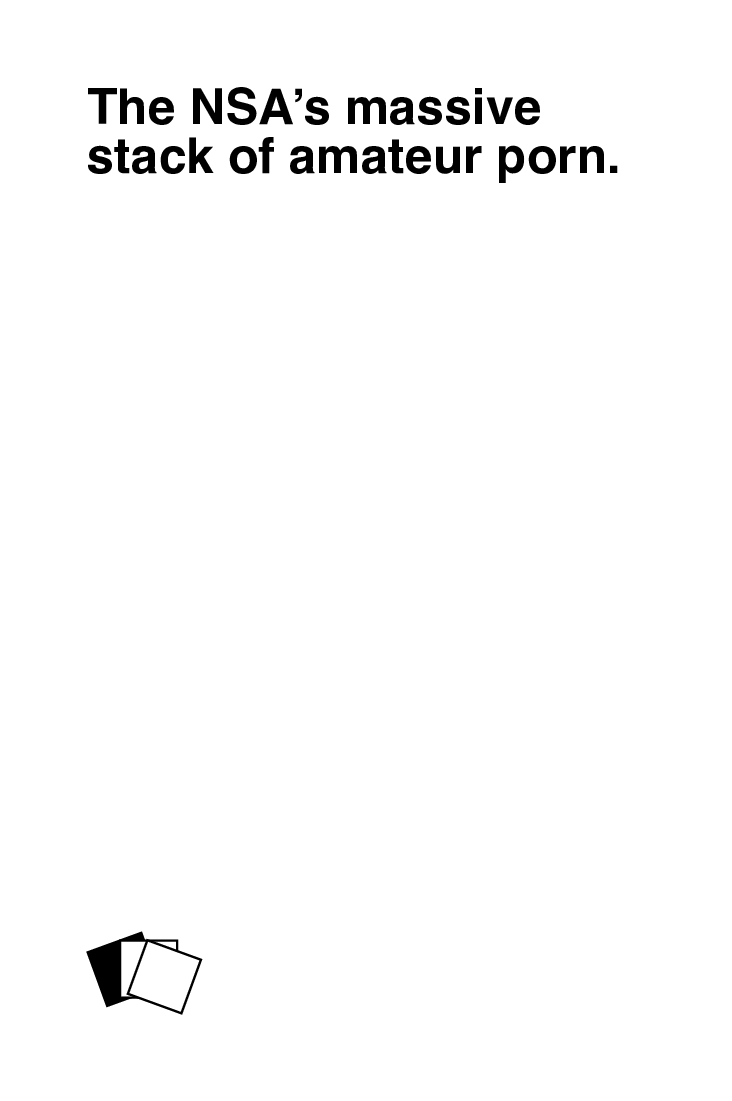
\includegraphics[width=.9\textwidth]{../zksummit/white_FRONT227.png}} % {CAC/PNGs-to-print/individual-cards/white_FRONT227.png}
	\end{column}
	\begin{column}[t]{0.3\textwidth}
	    \frame{
\includegraphics[width=.9\textwidth]{../zksummit/white_FRONT117.png}} % {CAC/PNGs-to-print/individual-cards/black_FRONT050.png}
    \end{column}
\end{columns}

\end{frame}


\begin{frame}{Are zk roll ups useful?}

\begin{enumerate}
\item Are teams capable of building zk roll ups useful? \\
 YES! \quad Attempt to lure them with availability, etc. \\ \medskip
% But.. \\ \medskip
\item What are the costs and latency of zk roll ups? \\
 % 1000x EC times 100x range proofs,  \\
 5 min on massive machines, with massive RAM \\ \medskip
\item What is the cost of polkadot? \\ \medskip
% \item Should we fund zk roll ups? \\ \medskip
\end{enumerate}

\end{frame}
 

\begin{frame}{How much can polkadot do?}

polkadot/issues/7324 mentioned Versi suffering under: \\ \medskip
% https://github.com/paritytech/polkadot/issues/7324#issuecomment-1600790000

\begin{tabular}{r c c c c}
validators (v)       & 200 & & \\
parachains cores (c) & 40  & & 120 & 100 \\
needed approvals (n) & 100 & & 33 & 40 \\
tranch 0 samples (z) & 30  & 20 & \\ % = 100 * 40 / 200 \\
\end{tabular}

\medskip 

Parachains are 50\% CPU burn, 50\% PoV size gluttons
 
Validators are potato VMs.  Babe not Sassafras.  etc.

$$ c (n - \sigma) \le z v \le c n  $$

\end{frame}

    
\begin{frame}{Goals: Batch verifiers}

Ephemeral storage \\ \bigskip

Schnorr \\ \bigskip

SnarkPack \\ \bigskip

zkAMMs like zkUniswap  \\ \bigskip

\hspace{10pt} Approximate zk roll ups?  Do we troll? \\ \bigskip

\end{frame}


\begin{frame}{Goals: Pseudo-academic}

Carrot: Multi-party computation (MPC) \\ \bigskip

MPC-in-the-head? Other MPCs? \\ \bigskip\bigskip

Inter-collator MPC? \\ \bigskip

User-collator(-user) MPC \\ \bigskip

\end{frame}


\begin{frame}{Goals: VRF games}

Users have (infinite) decks, aka a probability distribution \\ \medskip

An on-chain event produces secure-ish randomness, \\
\hspace{5pt} which fed through users VRFs represents their draws.

Users play the VRF signature when they choose to do so \\ \bigskip

\end{frame}


\begin{frame}{Goals: State-channel games}

First person shooters \\ \bigskip\bigskip

Real-time strategy \\ \bigskip\bigskip

\end{frame}


\end{document}







\begin{frame}
		
\end{frame}



\begin{frame}
	
\end{frame}




